\documentclass{article}
\usepackage{graphicx}
\usepackage{amsmath}
\usepackage{amssymb}
\usepackage[a4paper, top=25mm, bottom=25mm, left=25mm, right=25mm]{geometry}
\usepackage{pgfplots}
\pgfplotsset{compat=1.18}
\usepackage{mathtools}
\usepgfplotslibrary{polar}
\usepgfplotslibrary{fillbetween}

\begin{document}
\pagestyle{empty}
\large

\begin{center}
2024-2025 Spring \\MAT124 Midterm\\(09/04/2025)
\end{center}

\noindent 1. Consider the curve with the polar equation $r=2\cos(3\theta)$.

\hfill

\noindent (a) Find symmetry properties for the given curve and sketch the curve.

\hfill

\noindent (b) Find the area of the region enclosed by the curve.

\hfill

\noindent 2. Identify (describe and sketch) the following curves with polar equations using Cartesian coordinates.

\hfill

\noindent (i) $r=2\sin\theta +2\cos\theta$ \ \ \ (ii) $r=\tan\theta\sec\theta$

\hfill

\noindent 3.

\hfill

\noindent (a) The following vectors are given.
\[\mathbf{u}=6\mathbf{i}-3\mathbf{j}+2\mathbf{k}\quad\text{and}\quad\mathbf{v}=(4\mathrm{p}+1)\mathbf{i}+(\mathrm{p}-2)\mathbf{j}+\mathbf{k}\]

\noindent $\mathrm{p}$ is a scalar constant. Find the value of $\mathrm{p}$ if

\hfill

\noindent I. $\mathbf{u}$ and $\mathbf{v}$ are perpendicular vectors. \ \ \ \ \ II. $\mathbf{u}$ and $\mathbf{v}$ are parallel vectors.

\hfill

\noindent (b) The points $A(5,1,3),\:B(3,1,5),\:C(5,3,5)$ are given. Show that the triangle $\triangle{ABC}$ is equilateral and find its area.

\hfill

\noindent (c) Find the intersection of the line $L$ and the plane $R$.

\hfill

\noindent 4.

\hfill

\noindent (a) Find an equation of the plane through the point $P(1,2,3)$ parallel to the plane $R: x+y+z=1$.

\hfill

\noindent (b) Find the parametric equations of a line $L$ through the point $P(1,2,3)$ and perpendicular to the plane $R$.

\hfill

\noindent 5. Evaluate the limits, if they exist, and explain your answer.

\hfill

\noindent (a) $\displaystyle\lim_{(x,y)\to(0,0)}\frac{x^3y}{x^6+y^2}$ \ \ \ (b) $\displaystyle\lim_{(x,y)\to(0,0)}x^4\sin\left(\frac1{x^2+\left|y\right|}\right)$ \ \ \ 

\hfill

\noindent 6.

\hfill

\noindent (a) Find a vector function that represents the curve of intersection of two cylinders $x^2+y^2=1$ and $z=4x^2$.

\hfill

\noindent (b) Find the unit tangent vector to the curve in part (a) at $\displaystyle t=\frac\pi2$.

\hfill

\noindent (c) Find a formula for the length of the curve in part (a). Do not evaluate the length.

\hfill

\noindent 7. Use traces to sketch and identify the surface given by the equation $z=-x^2-y^2+2$.

\newpage

\begin{center}
2024-2025 Spring Midterm (09/04/2025) Solutions\\
(Last update: 29/08/2025 01:59)
\end{center}

\noindent 1.

\hfill

\noindent (a) Determine whether the graph is symmetric about the $x$-axis.

\[(r,\theta)\rightarrow r=2\cos(3\theta),\qquad (r,-\theta)\rightarrow r=2\cos(-3\theta)=2\cos(3\theta)\]

\hfill

\noindent $(r,\theta)$ is on the graph, and the graph is symmetric about the $x$-axis. Determine whether the graph is symmetric about the origin.

\[(r,\theta)\rightarrow r=2\cos(3\theta),\qquad (r,\theta+\pi)\rightarrow r=2\cos(-3(\theta+\pi))=-2\cos(3\theta)\]

\hfill

\noindent $(r,\theta+\pi)$ is not on the graph, and the graph is not symmetric about the origin. Determine whether the graph is symmetric about the $y$-axis.

\[(r,\theta)\rightarrow r=2\cos(3\theta),\qquad (r,\theta-\pi)\rightarrow r=2\cos(-3(\theta-\pi))=-2\cos(3\theta)\]

\hfill

\noindent $(r,\theta-\pi)$ is not on the graph, and the graph is not symmetric about the $y$-axis. 

\begin{center}
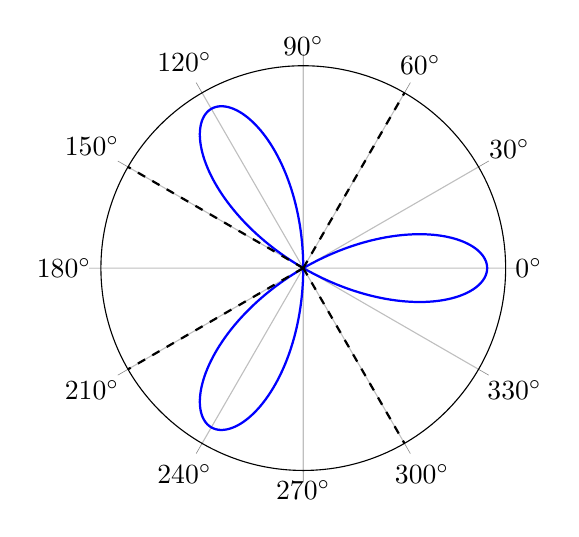
\begin{tikzpicture}
  \begin{polaraxis}[ytick=\empty, axis y line=none, xticklabel=$\pgfmathprintnumber{\tick}^\circ$,      scale=0.75,]
    \addplot [
      domain=0:2*pi,
      samples=300,
      thick,
      blue,
      data cs=polarrad,
    ] {2*cos(deg(3*x))};

    \draw[black, thick, dashed] (axis cs: 60,0) -- (axis cs: 60,2.5);
    \draw[black, thick, dashed] (axis cs: -60,0) -- (axis cs: -60,2.5);
    \draw[black, thick, dashed] (axis cs: 150,0) -- (axis cs: 150,2.5);
    \draw[black, thick, dashed] (axis cs: 210,0) -- (axis cs: 210,2.5);

  \end{polaraxis}
\end{tikzpicture}
\end{center}

\noindent (b) It is sufficient to calculate the area of the upper half of the leaf right to the $y$-axis and multiply the result by six.

\begin{center}
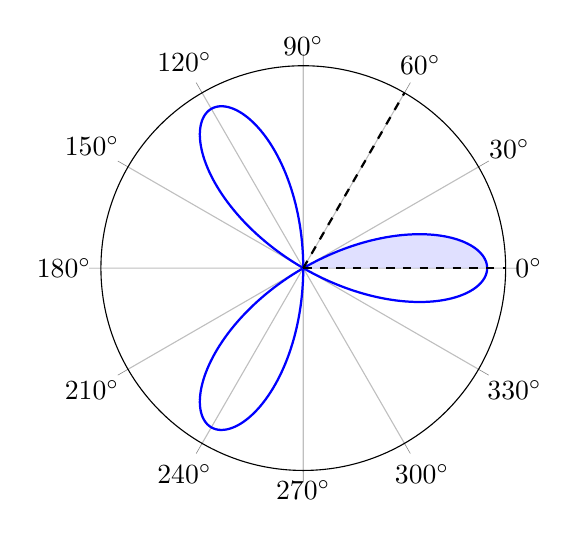
\begin{tikzpicture}
  \begin{polaraxis}[ytick=\empty, axis y line=none, xticklabel=$\pgfmathprintnumber{\tick}^\circ$,      scale=0.75,]
    \addplot [
      domain=0:2*pi,
      samples=300,
      thick,
      blue,
      data cs=polarrad,
    ] {2*cos(deg(3*x))};
    
    \addplot [
      domain=0:pi/6,
      draw=none,
      data cs=polarrad,
      name path=B
    ] {2*cos(deg(3*x))};
    
    \addplot [
      domain=0:pi/6,
      draw=none,
      data cs=polarrad,
      name path=A
    ] {0};
    
    \addplot [
      blue!20,
      fill opacity=0.6,
    ] fill between[of=A and B];

    \draw[black, thick, dashed] (axis cs: 60,0) -- (axis cs: 60,2.5);
    \draw[black, thick, dashed] (axis cs: 0,0) -- (axis cs: 0,2.5);

  \end{polaraxis}
\end{tikzpicture}
\end{center}
\begin{align*}\frac12\int_0^{\pi/6}\left(2\cos(3\theta)\right)^2\,d\theta&=\frac12\int_0^{\pi/6}4\cos^2(3\theta)\,d\theta=2\int_0^{\pi/6}\frac{1-\cos(6\theta)}2\,d\theta\\\\&=\left.\theta-\frac{\sin(6\theta)}6\right|_0^{\pi/6}=\frac\pi6\end{align*}

\hfill

\noindent The area is then
\[\text{Area}=6\cdot\frac\pi6=\boxed{\pi}\]

\hfill

\noindent 2.

\hfill

\noindent (i) Multiply each side by $r$.

\[r=2\sin\theta+2\cos\theta\implies r^2=2r\sin\theta+2r\cos\theta\]

\hfill

\noindent Using the equations $x=r\cos\theta$ and $y=r\sin\theta$, we get

\begin{align*}x^2+y^2=2x+2y&\implies x^2-2x+y^2+2y=0\implies x^2-2x+1+y^2-2y+1=2\\\\&\implies(x-1)^2+(y-1)^2=\left(\sqrt2\right)^2\end{align*}

\hfill

\noindent This is a circle with radius $\sqrt2$ centered at $(1,1)$.

\begin{center}
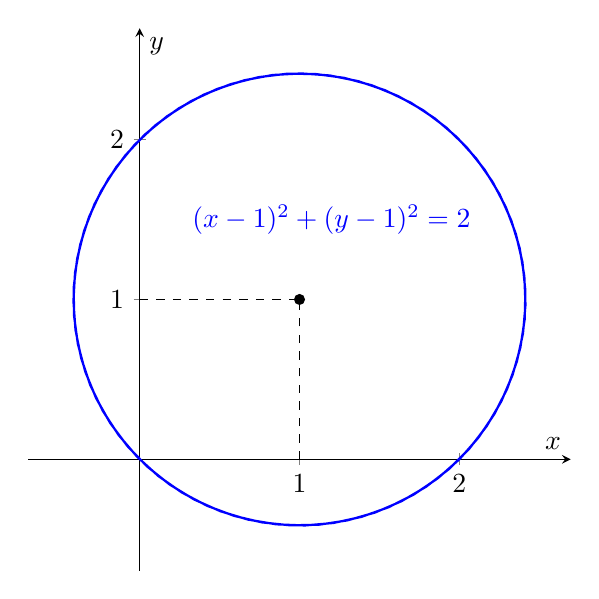
\begin{tikzpicture}
  \begin{axis}[
      axis lines = center,
      xlabel = {$x$},
      ylabel = {$y$},
      samples=100,
      xtick={1,2}, ytick={1,2},
      scale=1.21,
      axis equal image,
      enlargelimits=true,
    ]
    
    \addplot[blue, thick, domain=0:360] ({(2*sin(x)+2*cos(x))*cos(x)}, {(2*sin(x)+2*cos(x))*sin(x)});
    \fill (axis cs:1,1) circle (2pt);
    \node[blue] at (1.2,1.5) {$(x-1)^2+(y-1)^2=2$};
    \draw[dashed](1,0)--(1,1); \draw[dashed](0,1)--(1,1);
  \end{axis}
\end{tikzpicture}
\end{center}

\hfill

\noindent (ii) Rearrange the equation.

\[r=\tan\theta\sec\theta=\frac{\sin\theta}{\cos^2\theta}\implies r\cos^2\theta=\sin\theta\implies r^2\cos^2\theta=r\sin\theta\]

\hfill

\noindent Using the equations $x=r\cos\theta$ and $y=r\sin\theta$, we get the parabola $x^2=y$, where its branches open upward along the $y$-axis with the vertex $(0,0)$.

\begin{center}
\begin{tikzpicture}
  \begin{axis}[
      axis lines = center,
      xlabel = {$x$},
      ylabel = {$y$},
      samples=100,
      scale=1.21,
      axis equal image,
      enlargelimits=true,
    ]
    
    \addplot[blue, thick, domain=-2:2] {x^2};
    \node[blue] at (1.2,3) {$y=x^2$};
  \end{axis}
\end{tikzpicture}
\end{center}
\noindent 3.

\hfill

\noindent (a)

\hfill

\noindent (i) If $\mathbf u$ and $\mathbf v$ are perpendicular, the dot product of these vectors is equal to zero.

\[\mathbf u\cdot\mathbf v=\left\langle6,-3,2\right\rangle\cdot\left\langle4p+1,\,p-2,\,1\right\rangle=6(4p+1)-3(p-2)+2\cdot1=21p+14=0\implies p=\boxed{-\frac23}\]

\hfill

\noindent (ii) If $\mathbf u$ and $\mathbf v$ are parallel, the cross product of these vectors is equal to the zero vector.

\begin{align*}\mathbf{u}\times\mathbf{v}&=\left|\begin{array}{ccc}
\mathbf{i}&\mathbf{j}&\mathbf{k}\\
6&-3&2\\
4p+1&p-2&1
\end{array}\right|=\mathbf{i}\left|\begin{array}{cc}
-3&2\\p-2&1
\end{array}\right|-\mathbf{j}\left|\begin{array}{cc}
6&2\\4p+1&1
\end{array}\right|+\mathbf{k}\left|\begin{array}{cc}
6&-3\\4p+1&p-2
\end{array}\right|\\\\&=[1\cdot(-3)-2(p-2)]\mathbf i-(6\cdot1-2(4p+1))\mathbf j+[6(p-2)-(-3)(4p+1)]\mathbf k\\\\&=(1-2p)\mathbf i-(4-8p)\mathbf j+(-9+18p)\mathbf k=\mathbf0\implies \boxed{p=\frac12}\end{align*}

\hfill

\noindent (b) The sides of an equilateral triangle have the same length.

\[\overrightarrow{AB}=\left\langle3-5,\,1-1,\,5-3\right\rangle=\left\langle-2,0,2\right\rangle\rightarrow\left|\overrightarrow{AB}\right|=\sqrt{(-2)^2+0^2+2^2}=\sqrt8\]
\[\overrightarrow{AC}=\left\langle5-5,\,3-1,\,5-3\right\rangle=\left\langle0,2,2\right\rangle\rightarrow\left|\overrightarrow{AC}\right|=\sqrt{0^2+2^2+2^2}=\sqrt8\]
\[\overrightarrow{BC}=\left\langle5-3,\,3-1,\,5-5\right\rangle=\left\langle2,2,0\right\rangle\rightarrow\left|\overrightarrow{AC}\right|=\sqrt{2^2+2^2+0^2}=\sqrt8\]

\hfill

\noindent Half of the magnitude of the cross product of two vectors gives us the area of the triangle.

\[\frac12\left|\overrightarrow{AB}\times\overrightarrow{AC}\right|=\frac12\left|\overrightarrow{AB}\right|\left|\overrightarrow{AC}\right|\sin\frac\pi3=\frac12\cdot\sqrt8\cdot\sqrt8\cdot\frac{\sqrt3}2=\boxed{2\sqrt3}\]

\hfill

\noindent 4.

\hfill

\noindent (a) The planes have the same normal $\mathbf n=\left\langle1,1,1\right\rangle$. Using the definition $\mathbf n\cdot\overrightarrow{PP_0}=0$, we obtain

\[1(x-1)+1(y-2)+1(z-3)=0\implies\boxed{x+y+z=6}\]

\hfill

\noindent (b) The direction vector of the line is the normal vector of the plane. Therefore, the parametric equations for the line $L$ is as follows.

\[\boxed{\left.\begin{array}{l}
x=1+t\\
y=2+t\\
z=3+t
\end{array}\right\}\quad t\in\mathbb{R}}\]

\hfill

\noindent (c) Substitute the equation of $L$ in the equation of the plane $R$.

\[x+y+z=1\implies (1+t)+(2+t)+(3+t)=1\implies 3t+6=1\implies t=-\frac53\]
\[t=-\frac53\implies x=1-\frac53=-\frac23,\quad y=2-\frac53=\frac13,\quad z=3-\frac53=\frac43\]

\hfill

\noindent Therefore, the point of intersection is $\boxed{\left(-\frac23,\frac13,\frac43\right)}$.

\hfill

\noindent 5. 

\hfill

\noindent (a) Apply the Two-Path Test.

\[y=x\implies\lim_{(x,y)\to(0,0)}\frac{x^3y}{x^6+y^2}=\lim_{x\to0}\frac{x^4}{x^6+x^2}=\lim_{x\to0}\frac{x^2}{x^4+1}=\frac01=0\]
\[y=x^3\implies\lim_{(x,y)\to(0,0)}\frac{x^3y}{x^6+y^2}=\lim_{x\to0}\frac{x^6}{2x^6}=\lim_{x\to0}\frac12=\frac12\]

\hfill

\noindent Since $0\neq\dfrac12$, by the Two-Path Test, the limit does not exist.

\hfill

\noindent (b) We have the inequality $\left|\sin\theta\right|\leq1$ for all values of $\theta$. Therefore,

\[-1\leq\sin\left(\frac1{x^2+|y|}\right)\leq1\qquad\left[\text{except for }x=0,\,y=0\right]\]
\[-x^4\leq x^4\sin\left(\frac1{x^2+|y|}\right)\leq x^4\]

\[\lim_{(x,y)\to(0,0)}-x^4=\lim_{(x,y)\to(0,0)}x^4=0\implies\lim_{(x,y)\to(0,0)}x^4\sin\left(\frac1{x^2+|y|}\right)=\boxed0\]

\hfill

\noindent By the squeeze theorem, the limit is equal to zero.

\newpage

\noindent 6.

\hfill

\noindent (a) Parametrize the curve using $0\leq t\leq 2\pi$.

\[x=\cos t,\:y=\sin t,\:z=4\cos^2t,\qquad0\leq t\leq2\pi\]
\[\boxed{\mathbf r(t)=\left\langle\cos t,\,\sin t,\,4\cos^2t\right\rangle\qquad0\leq t\leq2\pi}\]

\hfill

\noindent (b) The tangent vector can be obtained by taking the first derivative of the vector function.

\[\mathbf T(t)=\mathbf r'(t)=\left\langle-\sin t,\,\cos t,\,-8\cos t\sin t\right\rangle\]

\hfill

\noindent The unit tangent vector is

\[\frac{\mathbf T(t)}{\left|\mathbf T(t)\right|}=\frac{\left\langle-\sin t,\,\cos t,\,-8\cos t\sin t\right\rangle}{\sqrt{(-\sin t)^2+(\cos t)^2+(-8\cos t\sin t)^2}}=\frac{\left\langle-\sin t,\,\cos t,\,-8\cos t\sin t\right\rangle}{\sqrt{1+64\cos^2t\sin^2t}}\]

\hfill

\noindent At $t=\dfrac\pi2$,

\[\frac{\mathbf T(t=\pi/2)}{|\mathbf T(t=\pi/2)|}=\frac{\left\langle-\sin\dfrac\pi2,\,\cos \dfrac\pi2,\,-8\cos\dfrac\pi2\sin\dfrac\pi2\right\rangle}{\sqrt{1+64\cos^2\dfrac\pi2\sin^2\dfrac\pi2}}=\boxed{\left\langle-1,0,0\right\rangle}\]

\hfill

\noindent (c) The length of the parametrized curve $\mathbf{r}(t)=\left\langle x(t),\,y(t),\,z(t)\right\rangle$ for $a\leq t\leq b$ can be evaluated using the integral

\[L=\int_a^b\left|\frac{d\mathbf r}{dt}\right|\,dt\]

\hfill

\noindent The length of the curve is then

\begin{align*}L&=\int_0^{2\pi}\left|\frac{d\mathbf r}{dt}\right|\,dt=\boxed{\int_0^{2\pi}\sqrt{1+64\cos^2t\sin^2t}\,dt=\int_0^{2\pi}\sqrt{1+16\sin^22t}\,dt}\end{align*}

\hfill

\noindent 7. This is a circular paraboloid with the vertex $(0,0,2)$ opening downward along the $z$-axis.

\begin{center}
\begin{tikzpicture}
  \begin{axis}[
  title={Plane $x=0$},
    xlabel=$y$, ylabel=$z$,
    xtick=\empty, ytick=\empty,
    samples=50,
    axis lines=middle,
    clip=true,
    scale=1,
    enlargelimits=true
    ]
    \addplot[domain=-5:5, blue] {-x^2/4+2};

    \node[blue] at (2.2,-2.8) {$z=-y^2+2$};
  \end{axis}
\end{tikzpicture}\hspace{1em}
\begin{tikzpicture}
  \begin{axis}[
  title={Plane $y=0$},
    xlabel=$x$, ylabel=$z$,
    xtick=\empty, ytick=\empty,
    samples=50,
    axis lines=middle,
    clip=true,
    scale=1,
    enlargelimits=true
    ]
    \addplot[domain=-5:5, red] {-x^2/4+2};

    \node[red] at (2.2,-2.8) {$z=-x^2+2$};
  \end{axis}
\end{tikzpicture}

\begin{tikzpicture}
  \begin{axis}[
  title={Plane $z=0$},
  axis equal image,
    xlabel=$x$, ylabel=$y$,
    xtick=\empty, ytick=\empty,
    samples=300,
    axis lines=middle,
    clip=true,
    scale=1,
    enlargelimits=true
    ]
    \addplot[domain=-sqrt(2):sqrt(2), orange] {sqrt(2-x^2)};
    \addplot[domain=-sqrt(2):sqrt(2), orange] {-sqrt(2-x^2)};

    \node[orange] at (0.7,0.2) {$x^2+y^2=2$};
  \end{axis}
\end{tikzpicture}\hspace{1em}
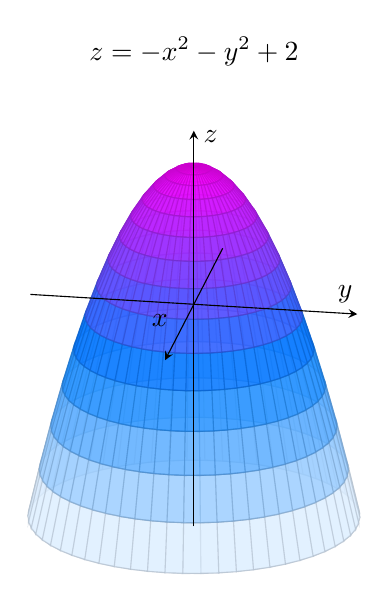
\begin{tikzpicture}
  \begin{axis}[
    title={$\displaystyle z=-x^2-y^2+2$},
    title style={yshift=-10pt},
      view={100}{20},
      axis lines=center,
      axis equal image,
      xlabel={$x$},
      ylabel={$y$},
      zlabel={$z$},
      domain=0:2*pi,
      y domain=-2.25:2.25,
      samples=30,
      samples y=30,
      colormap/cool,
      axis on top,
      scale=1.5,
      xtick=\empty, ytick=\empty, ztick=\empty,
      z buffer=sort,
      zmin=-3.2, zmax=2.5
    ]
    \addplot3[
      surf,
      opacity=0.6
    ]
    ({y*cos(deg(x))},
      {y*sin(deg(x))},
      {-y^2+2});
  \end{axis}
\end{tikzpicture}
\end{center}

\end{document}